\subsection{Combustor Model Validation - Stephen Kubicki}
A lumped parameter combustor model was created as a validation tool for the discretized combustor model discussed in \ref{CombustorModelingAndSim}. An important step in the design was to ensure the discretized model is calculating combustor behavior appropriately and providing accurate data for the SFRJ flight simulation. The lumped parameter model serves as a reliable comparison as it is a simpler model based on a few presiding assumptions, listed below. 

\begin{enumerate}
  \item Mach number is low throughout the combustor
  \item Combustor can be characterized by a single pressure
  \item Fuel grain burns at a single regression rate \\
\end{enumerate}

These assumptions combined lead to an important simplifying model assumption: axial variations in flow properties down the length of the combustor are ignored, so the entire combustor can be characterized by a single set of flow properties that varies with time. This makes the lumped parameter model akin to a discretized combustor model with a single axial section, the length of the combustor. The lumped parameter model is in many ways similar to the discretized combustor model described previously; the simulation is built as an independent function in the simulator environment, follows a similar flowpath loop as shown in Fig. \ref{fig:flowpath} (however without bypass modeling), and follows the same exact time iteration/pressure solving loop as described in Fig. \ref{fig:timeloop}. The time iteration of the lumped parameter combustor model will not be discussed in detail due to its similarity to the discretized combustor model, but the process and equations utilized to compute the updated flow properties will be described below. 

The lumped parameter model first pulls in the flow properties exiting the inlet pipe (mass flow rate, temperature, pressure, molecular weight, ratio of specific heats, etc.) and sets those as the flow properties in the entire combustor. The port area is computed based on the grain geometry at the current time step, and the Mach number in the combustor is computed to check if the flow is choked. The fuel regression rate is then found based on the oxidizer mass flux through the combustor and the regression rate constants for HTPB, as dicussed in \textbf{Reference ???}. Fuel mass flow rate can then be calculated based on the regression rate, the fuel density, and the exposed grain burn surface area (based on the grain geometry at the current time step). The oxidizer to fuel ratio, or O/F, is computed so CEA can be called using O/F and the current flow properties to simulate combustion, outputting updated properties for the entire chamber. Finally, the new total mass flow rate is calculated to recheck if the combustor is choked. Since axial variations in flow properties are ignored, this outlined process is repeated for each time step, pulling the initial flow properties from the inlet pipe each time and updating the grain geometry between iterations. The equations that this process describes are listed below. 

\begin{equation}
\centering   
M=\frac{\dot{m}_{ox}\sqrt{\frac{RT}{\gamma}}}{pA_p}
\end{equation}

\begin{equation}
\centering   
r=aG_{ox}^n=a(\frac{\dot{m}_{ox}}{A_p})^n
\end{equation}

\begin{equation}
\centering   
\dot{m}_f=r\rho_fA_b
\end{equation}

\begin{equation}
\centering   
O/F=\frac{\dot{m}_{ox}}{\dot{m}_f}
\end{equation}

\begin{equation}
\centering   
[flow,T_o,\gamma,C_p]=CEA(T,p,\frac{p_c}{p_e},O/F)
\end{equation}

\begin{equation}
\centering   
\dot{m}_{tot}=\frac{\dot{m}_{ox}}{\dot{m}_f}
\end{equation}

\begin{equation}
\centering   
M=\frac{\dot{m}_{tot}\sqrt{\frac{RT}{\gamma}}}{pA_p}
\end{equation}

The two combustor models were run in a static test stand simulation rather than a flight simulation in order to isolate the behavior of the models as much as possible, giving the best comparison of true behavior. Running the models in a flight simulation would lead to exaggerated divergence in behavior due to extra degrees of freedom in flight conditions. For example, consider a case where the two models were run in flight simulations beginning at the same initial flight conditions. A difference in combustor behavior can lead to cascading differences through the following: combustor behavior, performance parameters (i.e. thrust), vehicle dynamics, flight conditions, and flow properties through the inlet assembly. This process repeats each time step, with the properties of the two models diverging increasingly further as time progresses. The benefit of running the two models on a test stand is that it provides constant inlet conditions, hence isolating any possibility of the aforementioned cascading differences. Additionally, the two models were run without an AeroValve due to the fact that the lumped parameter model does not take into account axial variations in flow, so injecting bypass flow is not possible. Therefore, AeroValve flow was omitted to keep comparisons of the governing equations as close to 1:1 as possible. Finally, since the lumped parameter model uses a single set of flow properties to characterize the entire combustor, a set of flow properties from a discretized combustor section were selected (the aft-most section) to compare against. Flow properties from the static test stand runs for each of the combustor models are shown in Fig. \ref{fig:LPA_1} - Fig. \ref{fig:LPA_3} below.

\begin{figure}[H]
\centering
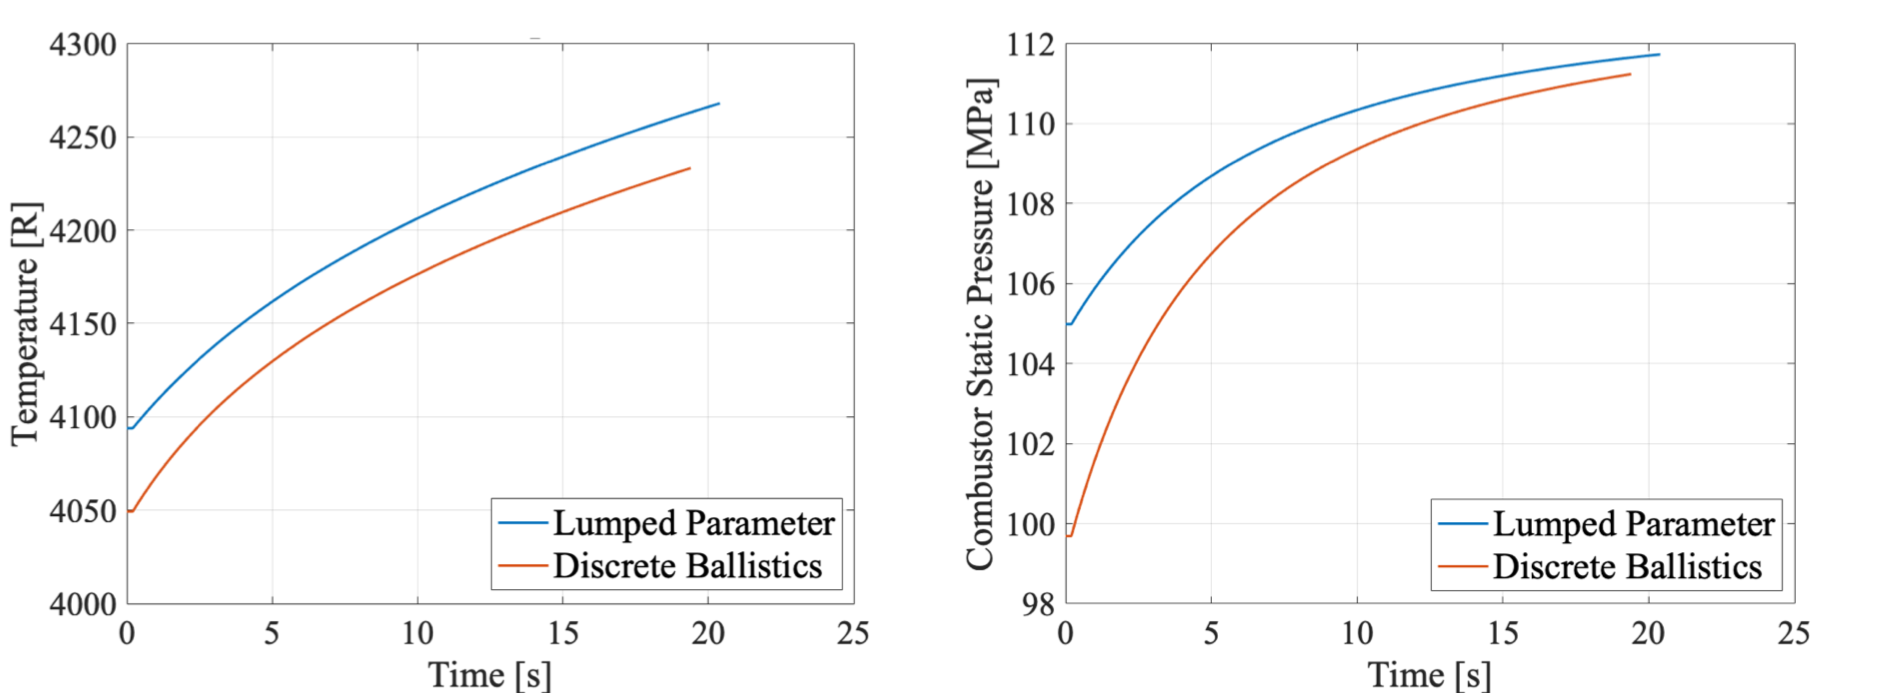
\includegraphics[width=1\textwidth] {Combustor_Figures/LPA_1.png}
\caption{Lumped Parameter Model - Static Temperature (Left) and Static Pressure (Right) vs. Time}
\label{fig:LPA_1}
\end{figure}

\begin{figure}[H]
\centering
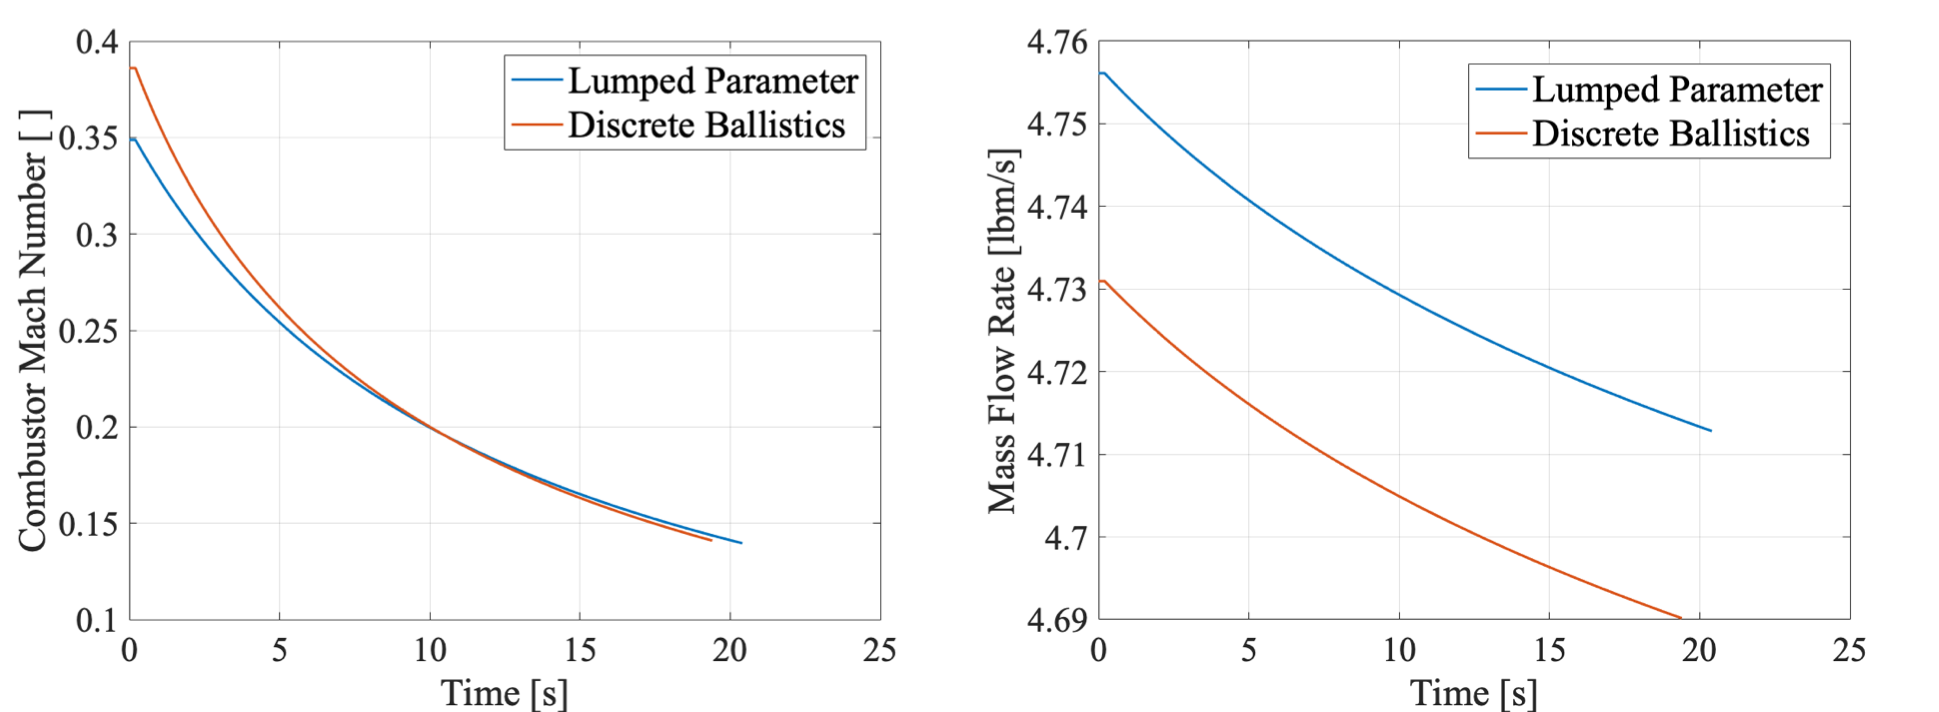
\includegraphics[width=1\textwidth] {Combustor_Figures/LPA_2.png}
\caption{Lumped Parameter Model - Mach Number (Left) and Mass Flow Rate (Right) vs. Time}
\label{fig:LPA_2}
\end{figure}

\begin{figure}[H]
\centering
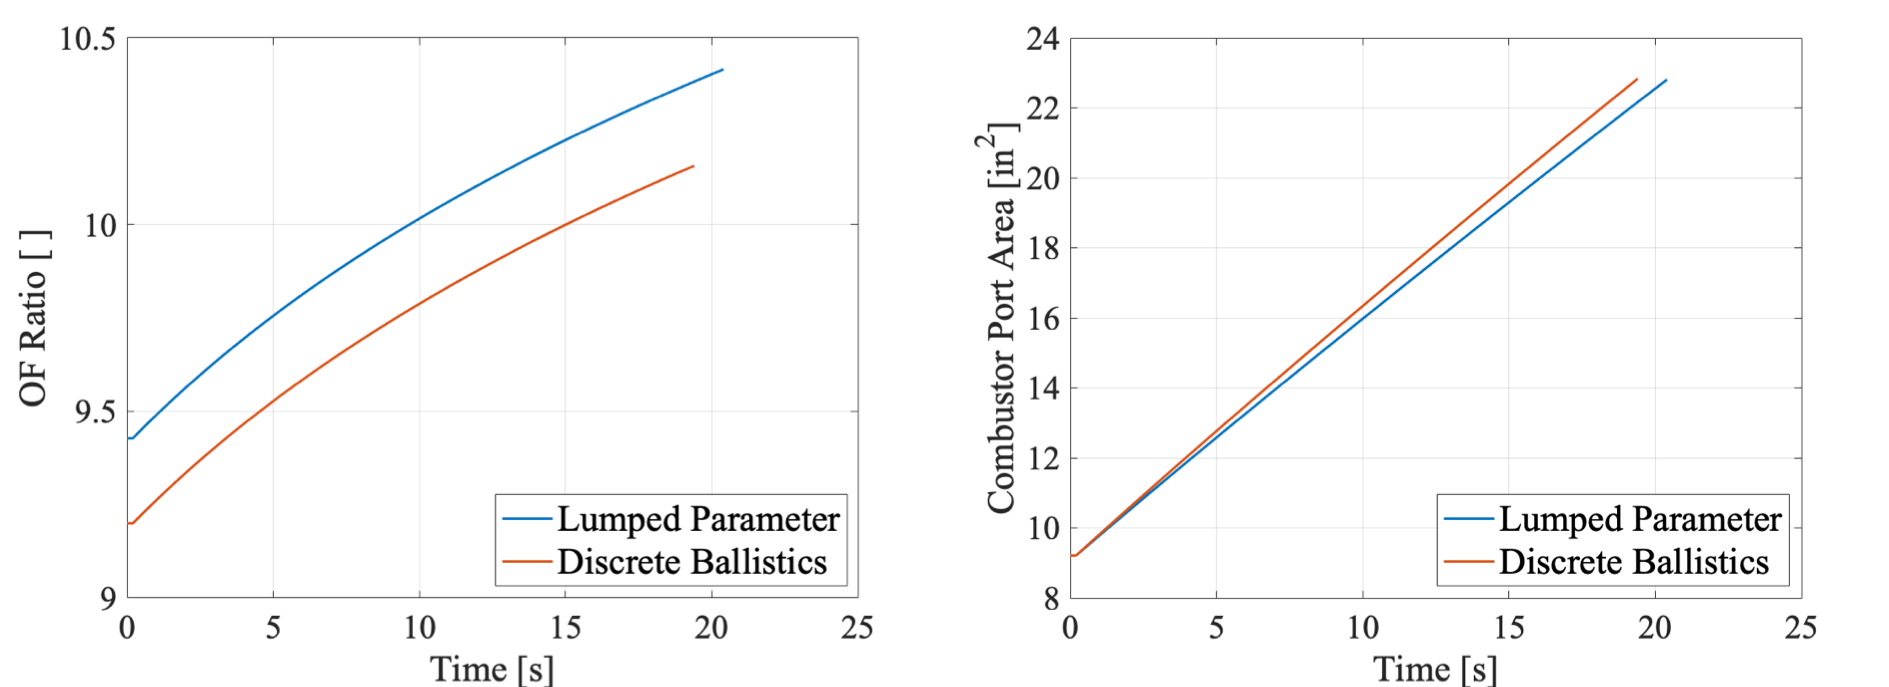
\includegraphics[width=1\textwidth] {Combustor_Figures/LPA_3.png}
\caption{Lumped Parameter Model - O/F (Left) and Port Area (Right) vs. Time}
\label{fig:LPA_3}
\end{figure}

A quick glance at these plots may make it appear that there is a marginal difference between the property time histories for the lumped parameter cobustor model and the discretized combustor model, however a closer inspection of the y-axes makes it clear that the two models behave in fairly close agreement. The average difference between the two models' properties are displayed in Table \ref{tab:LPAvsDiscrete}.

\begin{table}
    \centering
    \caption{Combustor Property Differences Between Models}
    \begin{tabular}{c|c}
    \textbf{Property} & \textbf{Difference [\%]} \\
    \hline
        Static Temperature & 0.8 \\ 
        Static Pressure & 1.5 \\ 
        Mach Number & 4.0 \\ 
        Mass Flow Rate & 0.5 \\ 
        O/F & 2.5 \\ 
        Port Area & 0.1
    \end{tabular}
    \label{tab:LPAvsDiscrete}
\end{table}

The initial conditions of the properties differ due to innate differences between the two models, particularly due to the fact that the properties update down the combustor length in the discretized model. Importantly, the trends of the properties appear to be consistent across the models, with difference between some properties being consistent with time while the rest converge with time. This provides good confidence that the discretized combustor model is used correctly and captures the combustor behavior appropriately, ultimately validating the model. Additionally, the plot of port area vs. time (Fig. \ref{fig:LPA_3} on the right) shows that both models reach the maximum port area, i.e. burn out, at nearly the same time, further supporting the validation of the model. 